%!TEX root = report.tex

\chapter{Results}

This chapter presents results from experiments 1, 2 and 3 as well as the
\texttt{ubus} smoke test and RSSI analysis. A discussion of these results will
follow in the subsequent chapter.

\section{Experiment 1}

The relation between computed $T_\text{delay}$, i.e. ($T_{pcap} - T_{sent}$), and
$T_\text{syscall}$ can be seen in Figure~\ref{fig:sysdelay}, where $T_{pcap}$
is the time reported by libpcap, $T_{sent}$ the timestamp right after
\texttt{sendto} returns and $T_{syscall}$ the time it took for \texttt{sendto}
to execute. This graph shows how our supposed ``packet sent timestamp'' was
dominated by the time it took to complete the call to \texttt{sendto}, which
could only block due to a full \texttt{sndbuf}.

\begin{figure}[tbp]
  \centering
  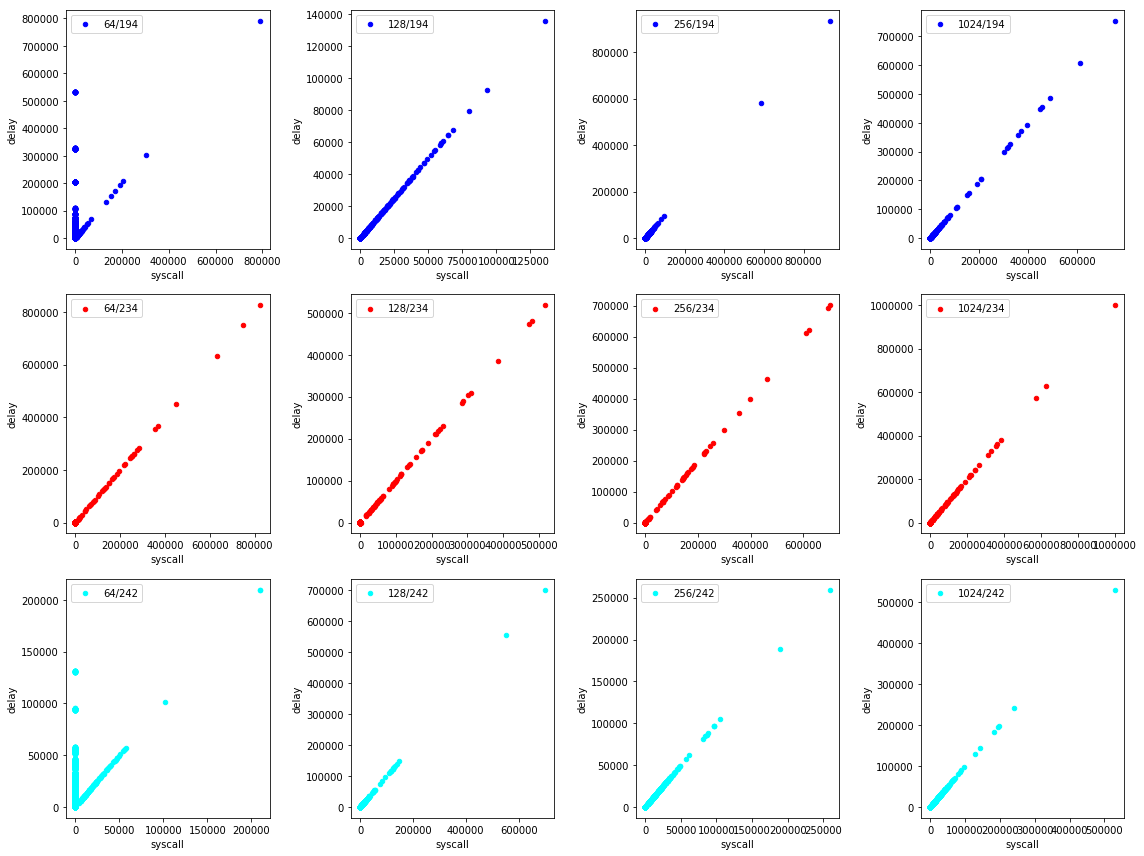
\includegraphics[width=1.2\textwidth]{images/delay-vs-syscall.png}
  \caption{Scatter plot of $T_\text{delay}$ and $T_\text{syscall}$ ($\mu s$) for each packet sent.
  Tests go from left to right, with each column being one test with a total of 3 different machines (and thus three rows).
  The first number in each legend is the packet payload size.}
  \label{fig:sysdelay}
\end{figure}

\section{Experiment 2}

In Table~\ref{tab:exp2data} we present the recorded NIC serve rate
$\lambda_{\mathtt{NIC}}$, \texttt{qdisc} queue length $L_{\mathtt{qdisc}}$,
specified \texttt{sndbuf} and packet \texttt{payload} size. The values were
obtained from a session with the system under test + 20 raspberry pi 4s.

\begin{table}[tbp]
  \centering
  \begin{tabular}{ll}
    $\lambda_{\mathtt{NIC}}$ & 4108 \\
    $L_\mathtt{qdisc}$ & 427 \\
    \texttt{sndbuf} & 1,5 MB \\
    payload & 1042 B
  \end{tabular}
  \caption{Average serve rate and estimated queue length of the NIC.}
  \label{tab:exp2data}
\end{table}

Recall from Equations~\ref{eq:sndbuf}~and~\ref{eq:wnic1} how
$L_{\mathtt{NIC}}$ can be obtained and used with Little's Law to estimate
$W_{\mathtt{NIC}}$:

\begin{align*}
L_{\mathtt{NIC}} &= \frac{\mathtt{sndbuf}}{\mathtt{payload} + \mathtt{overhead}} - L_\mathtt{qdisc} \approx \frac{1.5 \times 10^6}{1442} - 427 = 563 \\
W_\mathtt{NIC} &= \frac{L_{\mathtt{NIC}}}{\lambda_\text{NIC}} = \frac{563}{4108} = 137~ms
\end{align*}

Notice how $W_\mathtt{NIC}$ determines that under a fully loaded scenario, it
would take more than 100 \emph{milli}seconds to transmit 1 KB using UDP. Our
definition of \texttt{overhead}: IP + IEEE 802.11 + kernel bookkeeping.

\section{Experiment 3}

The final experiment was carried out on IEEE 802.11 \emph{n} (2.4 GHz) and
\emph{ac} (5 GHz). In Figures~\ref{fig:exp3throughput} and
\ref{fig:exp3mediatime} we present the total network throughput and
\texttt{wireless\_media\_time} for IEEE 802.11 \emph{n}. Similary, test
results for IEEE 802.11 \emph{ac} are shown in
Figures~\ref{fig:exp4throughput} and \ref{fig:exp4mediatime}.

Varying between each test is the number of actively participating clients as
well as their payload size. No specific packet generation distribution was
used, each client sent packets ``as fast as possible''.

It is important to note that, during this experiment, we could not control the
presence of nearby networks. However, the experiment was performed during
after-hours when no one was left at the office to run any traffic-heavy
applications. Additionally, any signficant traffic caused by unmanaged
software updates should show up as a significant outlier (much less
throughput, and higher \texttt{wireless\_media\_time}) for during an affected
experiment run.

In addition, running 60 tests ($15$ payload sizes $\times$ 4 host sizes) for
IEEE 802.11 $n$ \emph{and} $ac$, takes a couple of hours and should therefore
more easily show any temporary network impacts ony a single test run
(combination of active nodes and payload size) in the throughput graphs.

\begin{figure}[tbp]
  \centering
  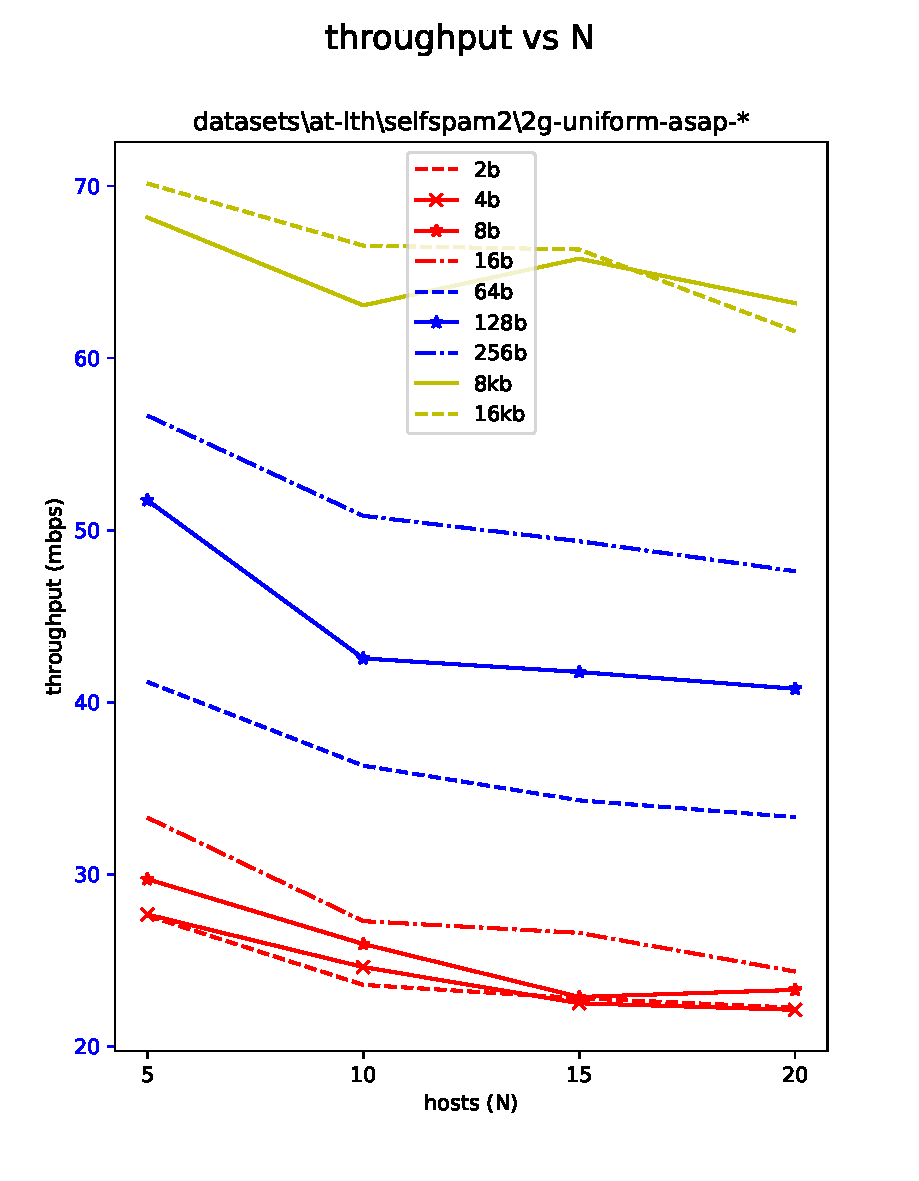
\includegraphics[width=0.8\textwidth]{images/exp3_tput.pdf}
  \caption{Experiment 3 - total network throughput (incl. UDP overhead) using IEEE 802.11 n.}
  \label{fig:exp3throughput}
\end{figure}

\begin{figure}[tbp]
  \centering
  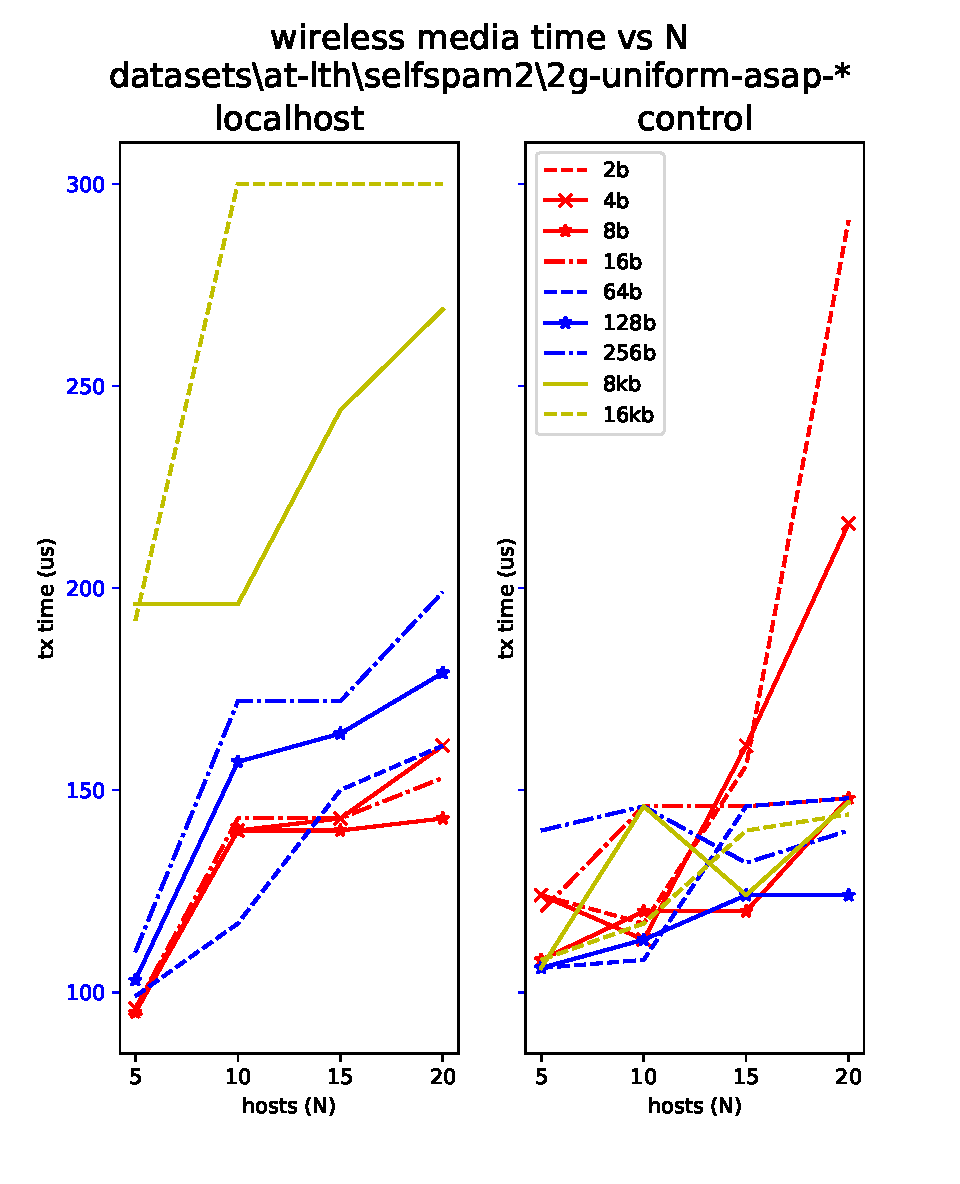
\includegraphics[width=0.65\textwidth]{images/exp3_wmt.pdf}
  \caption{Experiment 3 - wireless media tx time captured on two devices using IEEE 802.11 n.}
  \label{fig:exp3mediatime}
\end{figure}

\begin{figure}[tbp]
  \centering
  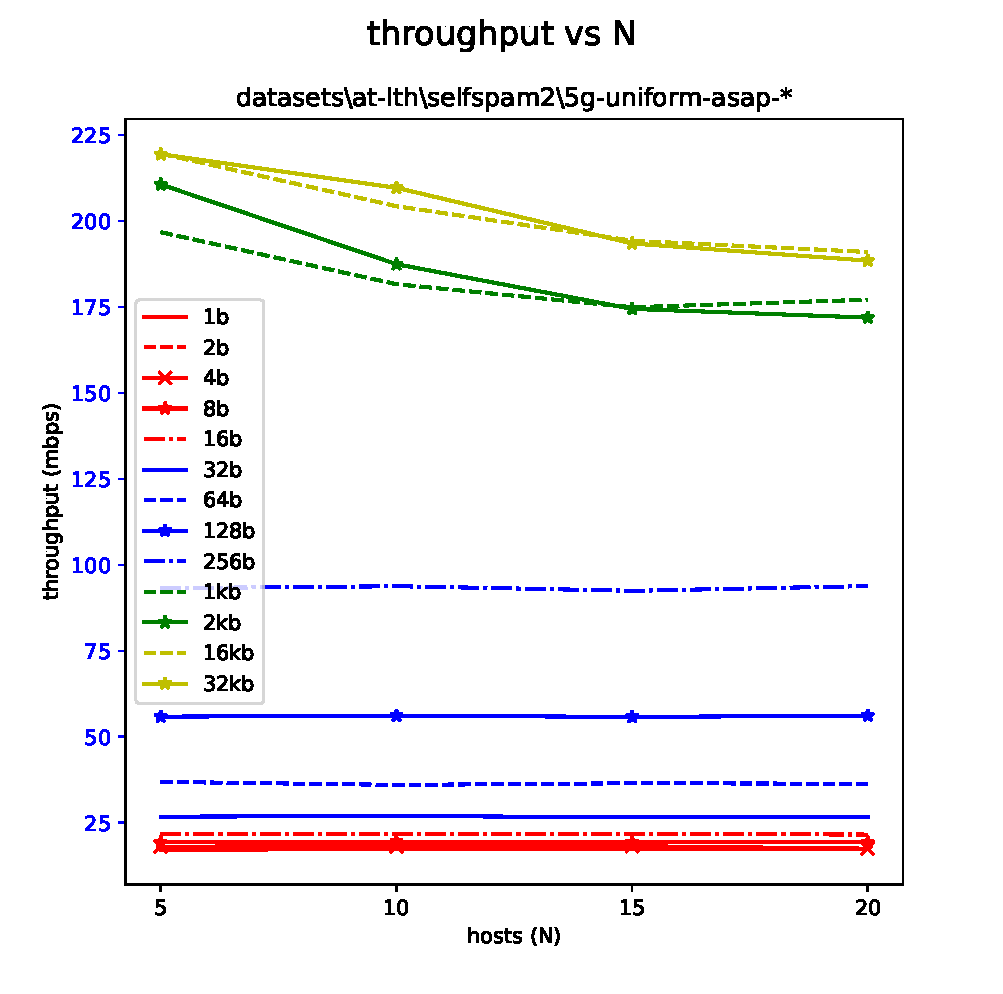
\includegraphics[width=0.8\textwidth]{images/exp4_tput.pdf}
  \caption{Experiment 3 - total network throughput (incl. UDP overhead) using IEEE 802.11 ac.}
  \label{fig:exp4throughput}
\end{figure}

\begin{figure}[tbp]
  \centering
  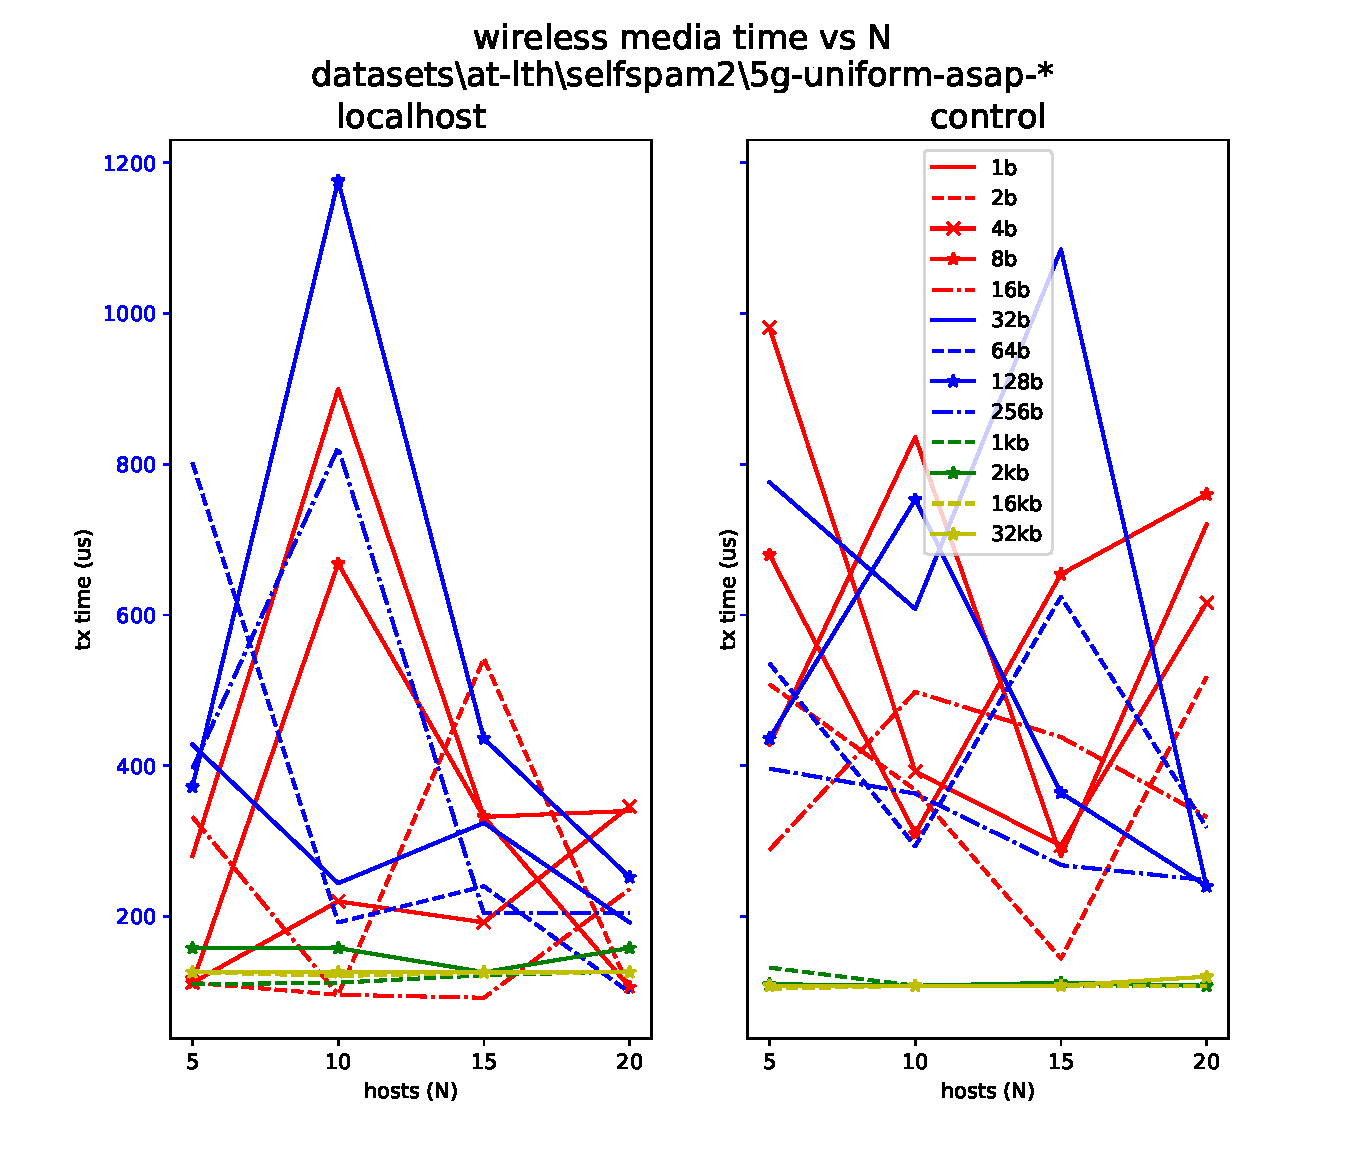
\includegraphics[width=0.8\textwidth]{images/exp4_wmt.pdf}
  \caption{Experiment 3 - wireless media tx time captured on two devices using IEEE 802.11 ac.}
  \label{fig:exp4mediatime}
\end{figure}

\section{\texttt{ubus} smoke test}

The \texttt{ubus} smoke test did not yield any presentable results, since most
of the test focused on verifying that no invalid data was returned.

No malformed output was noticed during our tests.

Inconsistencies on 5 GHz modem were first reported to us by Telenor, the 32-bit
byte counter did not overflow correctly and will get ``stuck'' at $2^{32} -
1$. Our findings initially showed similar behaviour for 2.4 GHz as well, but
was later attributed to a JSON conversion step (probably represented as signed
32 bit integers, instead of unsigned) in our logging approach.

This has been mitigated in our experiments by using byte counter values from
\texttt{iw} instead.

\section{RSSI}

Our RSSI experiment results are shown in Figure \ref{fig:rssiexpbaseline} and
\ref{fig:rssiexpsat}. Graphs show RSSI values as reported by the HF-6080
spectrum analyser, by sweeping the 802.11 ac spectrum in 1 MHz resolution.

Figure \ref{fig:rssiexpbaseline} shows the frequencies of the 802.11 ac
spectrum measurable by the device whereas Figure \ref{fig:rssiexpsat} only
shows frequencies for the (80 MHz) channel used.

RSSI values \emph{are} corrected for attenuation caused by the cable, average
of 6 dB across 802.11 ac frequencies, obtained from a Rohde \& Schwarz ZVL.

\begin{figure}[tbp]
  \centering
  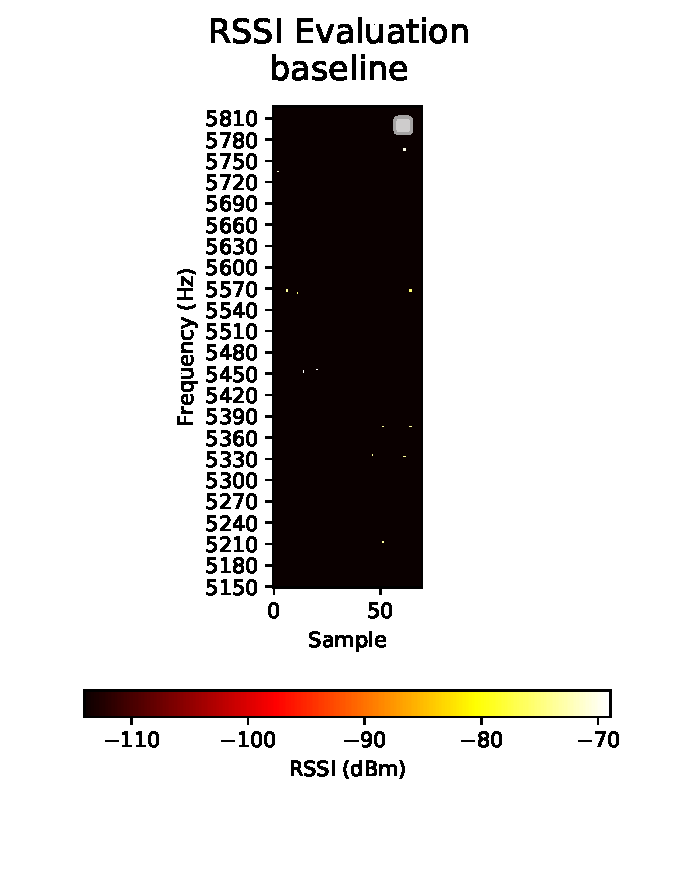
\includegraphics[width=0.7\textwidth]{images/rssi_baseline.pdf}
  \caption{RSSI baseline experiment, background activity.}
  \label{fig:rssiexpbaseline}
\end{figure}

\begin{figure}[tbp]
  \centering
  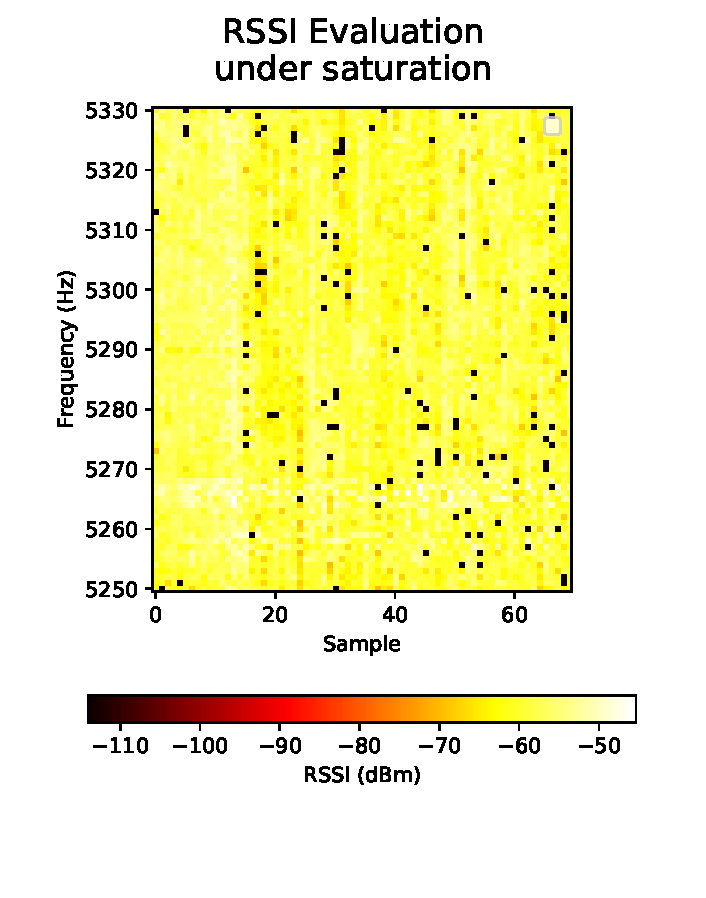
\includegraphics[width=0.8\textwidth]{images/rssi_under_load.pdf}
  \caption{RSSI experiment under iperf3 saturation using one 80 MHz channel.}
  \label{fig:rssiexpsat}
\end{figure}
